\documentclass[12pt]{article}
%Gummi|065|=)
\usepackage{amsmath, amsfonts, amssymb}
\usepackage[margin=0.5in]{geometry}
\usepackage{xcolor}
\usepackage{graphicx}
%\usepackage{graphicx}
\newcommand{\off}[1]{}
\DeclareMathSizes{20}{30}{20}{18}
\newcommand{\myhrule}{}

\newcommand{\two }{\sqrt[3]{2}}
\newcommand{\four}{\sqrt[3]{4}}

\newcommand{\dash}{
\begin{tikzpicture}[scale=1]
\draw (0,0)--(19,0);
\end{tikzpicture}
}

\newcommand{\sq}[3]{
\node at (#1+0.5,#2+0.5) {#3};
\draw (#1+0,#2+0)--(#1+1,#2+0)--(#1+1,#2+1)--(#1+0,#2+1)--cycle;
}

\usepackage{tikz}

\title{\textbf{Item: Riemann Integral}}
\author{John D Mangual}
\date{}
\begin{document}

\fontfamily{qag}\selectfont \fontsize{12.5}{15}\selectfont

\maketitle

\noindent In the math class we learn that Riemann sums converge to the Riemann integral.  
$$ \lim_{|\Delta x| \to 0} \sum_{i=0}^{N-1} f( x_i) \, \Delta x_i = \int_0^1 f(x) \, dx $$ 
where the interval $[0,1]$ has been partitioned into small intervals $[x_i, x_{i+1}]$.  \\ \\
There are doubts that I have from when I learned Real Analysis.  The most vanilla case of an integral is Area or Volume: any kind of \textbf{quadrature}. \\
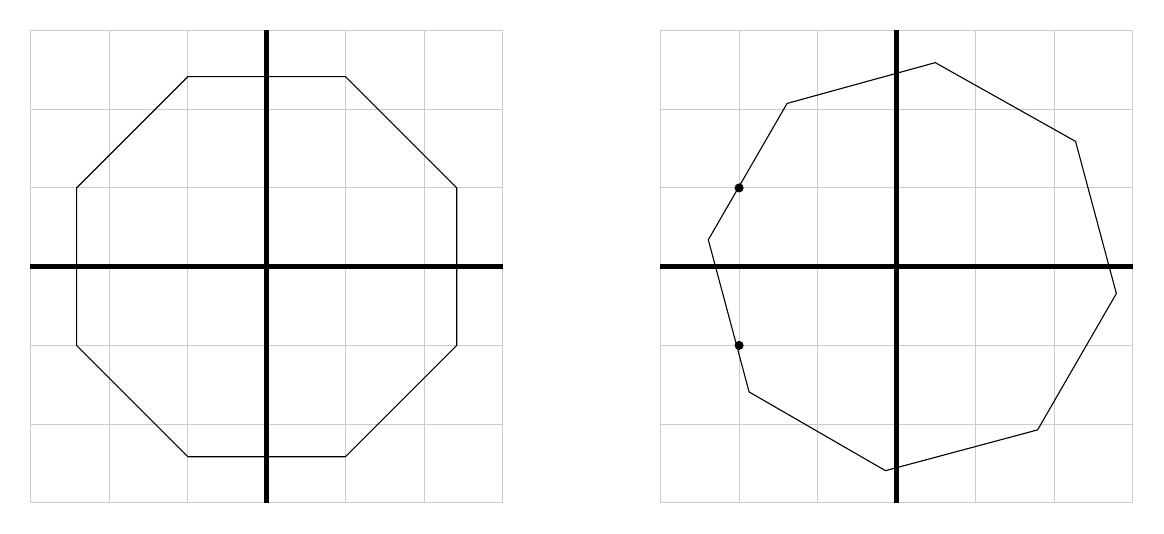
\begin{tikzpicture}

\begin{scope}[xshift=0]

\foreach \a in {-3,...,3}{
	\draw[color=black!20!white] (\a,-3)--(\a,3);
	\draw[color=black!20!white] (-3,\a)--(3,\a);
}

\draw (1,2.414)--(2.414,1)--(2.414,-1)--(1,-2.414)--(-1,-2.414)--(-2.414,-1)--(-2.414,1)--(-1,2.414)--cycle;

\draw[line width=2] (-3,0)--(3,0);
\draw[line width=2] (0,-3)--(0,3);

\end{scope}


\begin{scope}[xshift=8cm]

\foreach \a in {-3,...,3}{
	\draw[color=black!20!white] (\a,-3)--(\a,3);
	\draw[color=black!20!white] (-3,\a)--(3,\a);
}

\draw (2.073+0.2,1.591)--(2.591+0.2,-0.341)--(1.591+0.2,-2.073)--(-0.341+0.2,-2.591)--(-2.073+0.2, -1.591)--(-2.591+0.2, 0.341)--(-1.591+0.2, 2.073)--(0.341+0.15, 2.591)--cycle;

\draw[fill=black] (-2, 1) circle (0.05);
\draw[fill=black] (-2,-1) circle (0.05);

\draw[line width=2] (-3,0)--(3,0);
\draw[line width=2] (0,-3)--(0,3);

\end{scope}

\end{tikzpicture} \\
Let us push that to an extreme: all integrals are areas; all integrals are quadratures. \\ \\
\textbf{Q1} As a warm-up.  Does the rotated octagon (right) pass through the two marked points $(-2, \pm 1)$? \\ \\
We are going to compute the octagon by decomposing into squares (and chunks of squares).
\begin{itemize}
\item homology
\item scissors congruence
\end{itemize}
These are some buzzwords in the literture that correspond to this basic computation.  This is not the original example I had in mind, which had to do with this formula:
$$ \int_0^1 f(x) \, dx 
+ \int_0^1 g(x) \, dx = \int_0^1 \Big( f(x) + g(x) \Big) \, dx$$
Our $f(x)$ is very well behaved $f(x) \equiv 1$ everywhere.  So there is no issue yet.

\vfill

\fontfamily{qag}\selectfont \fontsize{12}{10}\selectfont

\begin{thebibliography}{}



\item  \dots

\end{thebibliography}


\end{document}